\documentclass[a4paper,english,cleveref, autoref]{lipics-v2019}
%This is a template for producing LIPIcs articles. 
%See lipics-manual.pdf for further information.
%for A4 paper format use option "a4paper", for US-letter use option "letterpaper"
%for british hyphenation rules use option "UKenglish", for american hyphenation rules use option "USenglish"
%for section-numbered lemmas etc., use "numberwithinsect"
%for enabling cleveref support, use "cleveref"
%for enabling cleveref support, use "autoref"

\usepackage{pgfplots}
\usepackage{tikz}
\usetikzlibrary{positioning}

\definecolor{backgroundgray}{rgb}{.94,.94,.94}
\definecolor{lightgray}{rgb}{.35,.35,.5}
\definecolor{darkgray}{rgb}{.2, .2, .2}
\definecolor{purple}{rgb}{0.65, 0.12, 0.82}

\newcommand{\secref}[1]{Section~\ref{#1} - \nameref{#1}}
\newcommand{\figref}[1]{Figure~\ref{#1}}
\newcommand{\coderef}[1]{Listing~\ref{#1}}

\lstdefinelanguage{JavaScript}{
  keywords={typeof, new, true, false, catch, function, return, null, catch, switch, var, if, in, while, do, else, case, break, undefined},
  keywordstyle=\color{black}\bfseries,
  ndkeywords={class, export, boolean, throw, implements, import, this},
  ndkeywordstyle=\color{black}\bfseries,
  identifierstyle=\color{darkgray},
  sensitive=false,
  comment=[l]{//},
  morecomment=[s]{/*}{*/},
  commentstyle=\color{lightgray}\slshape,
  stringstyle=\color{darkgray}\ttfamily,
  morestring=[b]',
  morestring=[b]"
}

\lstdefinelanguage{TypeScript}{
  keywords={typeof, new, true, false, catch, function, return, null, catch, switch, var, if, in, while, do, else, case, break, undefined},
  keywordstyle=\color{black}\bfseries,
  ndkeywords={class, export, boolean, throw, implements, import, this, declare, constructor, namespace, interface},
  ndkeywordstyle=\color{black}\bfseries,
  identifierstyle=\color{darkgray},
  sensitive=false,
  comment=[l]{//},
  morecomment=[s]{/*}{*/},
  commentstyle=\color{lightgray}\slshape,
  stringstyle=\color{darkgray}\ttfamily,
  morestring=[b]',
  morestring=[b]"
}

\lstset{
   backgroundcolor=\color{backgroundgray},
   extendedchars=true,
   basicstyle=\footnotesize\ttfamily,
   showstringspaces=false,
   showspaces=false,
   numbers=left,
   numberstyle=\footnotesize,
   numbersep=9pt,
   tabsize=2,
   breaklines=true,
   showtabs=false
}

\graphicspath{{./graphics/}}%helpful if your graphic files are in another directory

\bibliographystyle{plainurl}% the mandatory bibstyle

\title{Generation of TypeScript Declaration Files from JavaScript Code}

% \titlerunning{Dummy short title}%optional, please use if title is longer than one line

\author{John Q. Public}{Dummy University Computing Laboratory, Country \and My second affiliation, Country \and \url{http://www.myhomepage.edu} }{johnqpublic@dummyuni.org}{https://orcid.org/0000-0002-1825-0097}{(Optional) author-specific funding acknowledgements}%TODO mandatory, please use full name; only 1 author per \author macro; first two parameters are mandatory, other parameters can be empty. Please provide at least the name of the affiliation and the country. The full address is optional

\authorrunning{J.\,Q. Public}%TODO mandatory. First: Use abbreviated first/middle names. Second (only in severe cases): Use first author plus 'et al.'

\Copyright{John Q. Public}%TODO mandatory, please use full first names. LIPIcs license is "CC-BY";  http://creativecommons.org/licenses/by/3.0/

\ccsdesc[300]{Software and its engineering~Software notations and tools}
\ccsdesc[100]{Software and its engineering~General programming languages}%TODO mandatory: Please choose ACM 2012 classifications from https://dl.acm.org/ccs/ccs_flat.cfm 

\keywords{JavaScript, TypeScript, Dynamic Analysis, Declaration Files}%TODO mandatory; please add comma-separated list of keywords

\category{}%optional, e.g. invited paper

\relatedversion{}%optional, e.g. full version hosted on arXiv, HAL, or other respository/website
%\relatedversion{A full version of the paper is available at \url{...}.}

\supplement{}%optional, e.g. related research data, source code, ... hosted on a repository like zenodo, figshare, GitHub, ...

%\funding{(Optional) general funding statement \dots}%optional, to capture a funding statement, which applies to all authors. Please enter author specific funding statements as fifth argument of the \author macro.

% \acknowledgements{I want to thank \dots}%optional

%\nolinenumbers %uncomment to disable line numbering

%\hideLIPIcs  %uncomment to remove references to LIPIcs series (logo, DOI, ...), e.g. when preparing a pre-final version to be uploaded to arXiv or another public repository

%Editor-only macros:: begin (do not touch as author)%%%%%%%%%%%%%%%%%%%%%%%%%%%%%%%%%%
\EventEditors{John Q. Open and Joan R. Access}
\EventNoEds{2}
\EventLongTitle{42nd Conference on Very Important Topics (CVIT 2016)}
\EventShortTitle{CVIT 2016}
\EventAcronym{CVIT}
\EventYear{2016}
\EventDate{December 24--27, 2016}
\EventLocation{Little Whinging, United Kingdom}
\EventLogo{}
\SeriesVolume{42}
\ArticleNo{23}
%%%%%%%%%%%%%%%%%%%%%%%%%%%%%%%%%%%%%%%%%%%%%%%%%%%%%%

\begin{document}

\maketitle

%TODO mandatory: add short abstract of the document
\begin{abstract}
Developers are starting to write complex and large JavaScript applications in TypeScript, a typed superset of JavaScript. TypeScript applications integrate JavaScript libraries by including typed descriptions of their APIs called declaration files. These files are maintained manually, which is error prone and highly time consuming. Discrepancies between a declaration file and the JavaScript implementation will prevent developers from using them.

This work presents \lstinline[language={}]!dts-generate!, a tool that generates a declaration file for JavaScript libraries uploaded to the NPM registry. It executes the library, gathers run-time information from the code examples written by the developers and generates the declaration file based on it. 244 declaration files were generated and compared against DefinitelyTyped, the standard public repository for declaration files. 33 files out of 244 had no differences.
\end{abstract}

\section{Introduction}
JavaScript has become the most popular language for writing web applications \cite{github-statistics}. It is also gaining popularity for back-end applications running in NodeJS. Its dynamic typing speeds up programming enabling developers to create simple pieces of code very fast, making JavaScript a very appealing programming language.

JavaScript is being used for creating complex and large applications. However, JavaScript was not intended to be more than a scripting language. Maintaining and evolving large JavaScript codebases is notably challenging. Mistakes such as mistyped property names and misunderstood or unexpected type coercion cause developers to spend a significant amount of time in debugging sessions. A JavaScript code blog\footnote{https://wtfjs.com} compiles experiences from developers facing unexpected situations while programming in JavaScript. \coderef{code:introduction-javascript-wtfs} exposes some of these unintuitive JavaScript behaviors.

\begin{lstlisting}[
    caption={\textbf{Unexpected JavaScript behavior} - falsy values, \lstinline!typeof!, \lstinline!null! and \lstinline!undefined! operators and type coercion.},
    language=JavaScript,
	label=code:introduction-javascript-wtfs,
    float,
    abovecaptionskip=-\medskipamount
]
"0" == false; // true
true == "1.00"; // true
false == "    \n\r\t     "; // true
false == []; // true
0 == []; // true
null == undefined; // true
"01" < "00100"; // false
[1] + 1; //'11'
[2] == "2"; // true
null + undefined + [1, 2, 3] // 'NaN1,2,3'
"hello world".lenth + 1 // NaN | note 'lenth' instead of 'length'
[1, 15, 20, 100].sort() // [ 1, 100, 15, 20 ]
typeof null; // object
null instanceof Object; // false
\end{lstlisting}

The overhead produced by such dynamic typing is not present in other languages that use build tools based on type information. The situation motivated the creation of TypeScript, a superset of JavaScript with typed annotations \cite{typescript}. It has become a widely used alternative among JavaScript developers, since it incorporates features that are helpful for developing and maintaining large applications \cite{DBLP:conf/icse/GaoBB17}. TypeScript enables the early detection of run-time errors detection and the integration of code intelligence tools like auto-completion in the IDEs.

Existing JavaScript libraries can be used in a TypeScript project by adding a declaration file that contains a typed description of the library's API. Declaration files are stored in a repository called DefinitelyTyped that contains declaration files for more than 6000 JavaScript libraries \cite{definitely-typed-repository}. Unfortunately, declaration files need to be manually created and maintained, which is error prone and time consuming. TypeScript does not perform any run-time check on these declaration files. A discrepancy between the declaration file and its corresponding JavaScript library would lead to additional frustration and debugging sessions, since type checks and code-intelligence features would be inaccurate.

Some previous work tackled the problem of automatically searching for mismatches between a declaration file and implementation code \cite{DBLP:conf/oopsla/FeldthausM14}. TSTest adapted the feedback-directed random testing technique, mainly used for testing Java libraries, to detect discrepancies between a declaration file and a JavaScript library \cite{DBLP:journals/pacmpl/KristensenM17}. Tools like TSInfer and TSEvolve are designed for assisting the creation of new declaration files and supporting the evolution the declaration file when the corresponding JavaScript library gets modified \cite{DBLP:conf/fase/KristensenM17}, respectively. TypeScript itself developed \lstinline[language={}]{dts-gen}, a tool that generates a declaration file that is meant to be used only as a `starting point for writing a high-quality declaration file' \cite{dts-gen}.

We explore in this work the possibilities for improving the existing tools. We present the tool \lstinline[language={}]{dts-generate}. It is based on an architecture that supports the generation of declaration files for an existing JavaScript library published to the NPM registry. The tool will gather data flow and type information at run-time and generate a declaration file based on that information.

The architecture supports the future incorporation of a Symbolic Execution Engine that expands the initial code base using the signatures in the declaration file. The iterative process of exploring new execution paths will refine the generated declaration file in each iteration.

Finally, we generated declaration files for 244 JavaScript libraries and evaluated them against DefinitelyTyped.

The contributions of this paper are as follows.
\begin{itemize}
    \item We introduce an architecture that supports generating TypeScript Declaration Files for a given JavaScript Library using run-time information. The architecture supports the future incorporation of a Symbolic Execution Engine that expands the initial code base using the signatures in the declaration file. The iterative process of exploring new execution paths will refine the generated declaration file in each iteration.

    \item We present the tool \lstinline{dts-generate}, a command line application that generates a valid TypeScript Declaration File for a specific NPM package using run-time information.

    \item Next, we deliver a test framework that supports generating a TypeScript Declaration File using \lstinline{dts-generate} for all JavaScript libraries in the DefinitelyTyped Repository. We present the results of running \lstinline{dts-generate} for 244 of these libraries.

    \item Finally, we present a TypeScript Declaration Files parser and comparator. Both tools were necessary for evaluating the results against DefinitelyTyped.
\end{itemize}

\section{Motivating Examples}

\section{dts-generate - Generation of TypeScript Declaration Files}
We introduce \lstinline{dts-generate}, a command line tool which generates a valid TypeScript Declaration File for a specific JavaScript Library uploaded to the NPM Registry, as explained in \figref{fig:tsd_generation_method_block_diagram}. The tool is intended to be used on existing, published \lstinline{npm} packages. The generated output TypeScript declaration file is a valid file which can be used for development and uploaded to the DefinitelyTyped Repository.

\begin{figure}[tp]
    \centering
    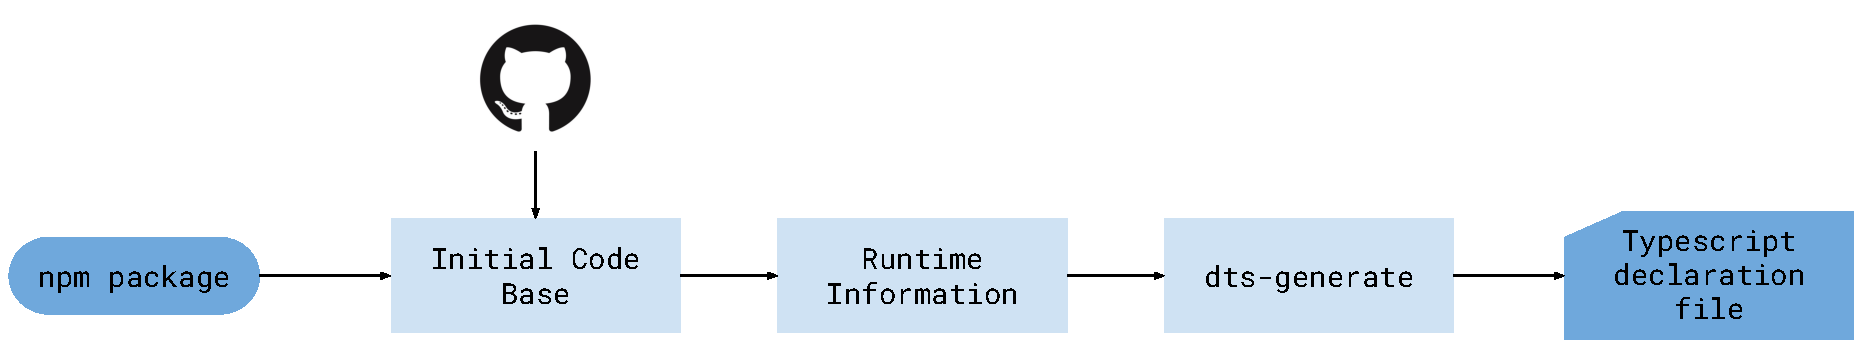
\includegraphics[width=1\linewidth]{dts-generate-block-diagram.pdf}
    \caption[dts-generate - Architecture overview]{\textbf{dts-generate - Architecture overview} - Initial code base is retrieved from the npm package's repository. A valid TypeScript Declaration File is generated using run-time information. A Symbolic Execution Engine creates test cases based on the generated Declaration File and via a feedback loop enriches the code base until the stopping criteria is reached. The final TypeScript Declaration File gets returned. Feedback loop through the Symbolic Execution Engine was not implemented. It can be added in a future to the existing architecture, without modifying the working blocks.}
    \label{fig:tsd_generation_method_block_diagram}
  \end{figure}

Code examples that execute the JavaScript Library are needed in order to extract the run-time information via code instrumentation. It is achieved by retrieving the examples provided in the README files of the repositories of the different libraries. This is generally the place where developers explicitly show how to use their code. It showed to be an appropriate and pragmatic way of extracting the developer's intention and providing an useful initial code base with meaningful examples, thus avoiding a possible cold start problem. 

The examples and the code base of the library are instrumented with Jalangi \cite{DBLP:conf/sigsoft/SenKBG13}\cite{DBLP:conf/sigsoft/SenKBG13a} to gather data flow information and type information at runtime. Jalangi is a dynamic analysis configurable framework that provides several analysis modules that were extended as needed to retrieve the required run-time information, which is then saved to an output JSON file.

A second independent block uses the run-time information to generate a TypeScript Declaration File. It infers the overall structure of the JS Library, the interfaces and the types from the JSON file.

The declaration file returned by the method is valid and fully functional, making it suitable for being used within the development process. It contains no errors and matches the structure of the JavaScript Library under analysis, so that the JavaScript code generated after compiling the TypeScript code runs without errors. The conducted experiments included tests that consisted on replacing a specific type definition from DefinitelyTyped \cite{definitely-typed-repository} with the one generated in the experiments: TypeScript compilation was successful, the generated JavaScript code ran without errors and code intelligence features performed by IDEs like code completion worked as expected.

The command line interface was inspired in the \lstinline{dts-gen} \cite{dts-gen} package. It can be seen in \coderef{code:dts-generate-example} that invoking the package is very simple and the only required argument is the name of the module published to the npm registry.

\begin{lstlisting}[
    caption={\textbf{dts-generate usage} - Example of how to generate a declaration file for module \lstinline{abs}.},
    language=bash,
	label=code:dts-generate-example,
    float,
    abovecaptionskip=-\medskipamount
]
$ ./dts-generate abs
$ cat output/abs/index.d.ts 
export = Abs;

declare function Abs(input: string): string;
\end{lstlisting}

\subsection{Initial Code Base}
To extract run-time information of a JavaScript Library, it is necessary, by definition, to actually execute the code, since the analysis modules provided by Jalangi to gather information are only triggered if the instrumented code gets executed.

It was decided to extract the code examples that execute the JavaScript Library from the Readme files of the repository associated to the NPM Package. Readme files are usually used by developers for briefly describing what the code does, what problem it solves, how to install the application, how to build the code, etc. It is very common that developers provide code examples in the readme files to show how the code works and how to use it. This is specially true for NPM Packages, which are in general created to solve a specific problem of JavaScript development.

Obtaining code examples for a specific NPM Package is achieved in three steps:
\begin{itemize}
  \item Obtain the repository url from the package: The command \lstinline{npm view <PACKAGE> repository.url} can be used for retrieving the url of the package's repository.

  \item Retrieve the README file from the repository.

  \item Extract the code examples from the README file: Readme files are written using Markdown\footnote{https://www.markdownguide.org}, a very common lightweight and simple markup language. It is very common to write code examples within code blocks indicating the programming language, so that it gets highlighted with the specific syntax. The Markdown identifiers for JavaScript are \lstinline{js} or \lstinline{javascript}. The code examples are finally retrieved by filtering the content within the corresponding code blocks.
\end{itemize}

\subsection{Run-time Information Gathering}
The Runtime Information block described in \figref{fig:tsd_generation_method_block_diagram} will gather information such as:

\begin{itemize}
  \item Function \lstinline{f} got invoked with parameters \lstinline{a} and \lstinline{b} with types \lstinline{string} and \lstinline{number}.
  \item Property or method \lstinline{foo} of parameter \lstinline{a} of function \lstinline{f} was accessed within the function.
  \item Parameter \lstinline{a} of function \lstinline{f} was used as operand for operator \lstinline{==}.
\end{itemize}

The dynamic analysis framework used for gathering this kind of information is Jalangi. The configurable analysis modules enable programming custom callbacks that get triggered with virtually any JavaScript event. The events that are observed are:
\begin{itemize}
  \item Binary operations, like \lstinline{==}, \lstinline{+} or \lstinline{===}.
  \item Variable declaration.
  \item Function, method, or constructor invocation.
  \item Access to an object's property.
  \item Unary operations, like \lstinline{!} or \lstinline{typeof}.
\end{itemize}

The implementation stores these observations as entities called \lstinline{interactions}. They are used for translating, modifying and aggregating Jalangi's raw event information in order to get an application specific data representation. The run-time information is finally returned as a JSON file that can be used for later processing. The tool is written in JavaScript and runs in Node.js within a Docker container.

\subsection{TypeScript Declaration File Generation}
\paragraph*{Overwiew}
The actual generation of the declaration file is the next step in the pipeline after gathering the run-time information, as shown in \figref{fig:tsd_generation_method_block_diagram}. It is a lightweight, simple and fast application, which does not interact with the actual JavaScript module at run-time. Instead, it uses the JSON output file containing the run-time information and generates a TypeScript declaration file which is use ready to be used within a TypeScript project. The tool itself is written in TypeScript and runs within a Docker container in NodeJS. 

\paragraph*{Templates}
TypeScript provides templates for writing declaration files\footnote{https://www.typescriptlang.org/docs/handbook/declaration-files/templates.html} and each template corresponds to a different way of exporting a JavaScript module. The tool uses different fields from the run-time information to detect how the module is being used in order to choose the right templates accordingly. The implemented templates are \lstinline{module}, \lstinline{module-class} and \lstinline{module-function}.

\paragraph*{Interfaces}
Finally, interfaces are created by exploring \lstinline{getField} and \lstinline{methodCall} interactions from the run-time information. The code will gather the interactions for a specific argument and build the interface by incrementally adding new properties. Interactions within the \lstinline{followingInteractions} field are recursively traversed, building a new interface in each recursion level.

\subsection{Evaluation}
\label{sec:dts-generate-evaluation}
After generating a declaration file for a published NPM module, it is necessary to evaluate the quality of it. It was decided to compare the generated declaration file against the one uploaded to the DefinitelyTyped repository for the same module, as shown in \figref{fig:evaluation-diagram}.

\begin{figure}[tp]
    \begin{centering}
        {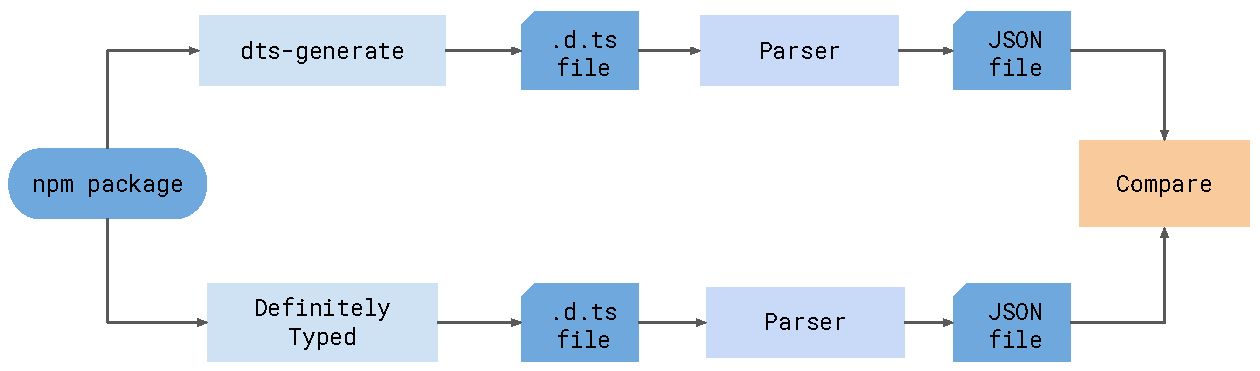
\includegraphics[width=1\textwidth]{evaluation-diagram.pdf}}
        \caption[Evaluation against DefinitelyTyped Repository]{\textbf{Evaluation of generated declaration files against DefinitelyTyped Repository} - A parser transforms the generated declaration file and the equivalent file in the DefinitelyTyped repository into a JSON file using the TypeScript Compiler API \cite{typescript-compiler-api}. Comparison is then performed on the JSON files, i.e. not on the declaration files.}
        \label{fig:evaluation-diagram}
    \end{centering}
\end{figure}

\paragraph*{Parsing}
Before comparison, declaration files need to be parsed so that both of them share the same structure. It was achieved by using the TypeScript Compiler API, a library developed by Microsoft that allows to traverse the Abstract Syntax Tree in an easy and intuitive way \cite{typescript-compiler-api}.

The parsing consists in creating a structure where declared \lstinline{interfaces}, \lstinline{functions}, \lstinline{classes} and \lstinline{namespaces} are stored separated. Function arguments are correctly described, identifying complex types like union types or callbacks. Optional parameters are also identified. For \lstinline{classes}, a distinction between the constructor and methods is made. Finally, syntax and semantic errors are also checked by the TypeScript Compiler API.

The tool is called \lstinline{parse-dts} and is naturally written in TypeScript. It also runs in NodeJS within its corresponding Docker container.

\paragraph*{Comparator}
An independent tool will compare two parsed declaration files. As described in \figref{fig:evaluation-diagram}, the comparator will compare the generated declaration file against the corresponding file in the DefinitelyTyped repository.

It was discovered that the implementation was easier when focusing on each template independently. For this implementation, only the \lstinline{module-function} was considered for the comparison.

The following criteria were applied:
\begin{itemize}
  \item Number of declared functions: Checks the number of declared and exported functions for each of both declaration files.
  \item Name of declared functions: Checks whether both of the declaration files declared a function with the same name.
  \item Number of parameters: Checks the number of parameters of the declared functions. This is checked for optional and non-optional parameters.
  \item Interfaces: Checks the number of declared interfaces and the fields within those interfaces.
  \item Errors: Indicates whether there are errors in the declaration files.
\end{itemize}

\section{Results}
Declaration files were generated for existing modules uploaded to the NPM registry. The DefinitelyTyped repository was used as a benchmark. Each one of the generated files was compared against the corresponding declaration file already uploaded to the repository.

Figure \ref{fig:experiments-overall-funnel} shows that a declaration file was generated for 244 modules out of 6029 modules. Samples of the generated declaration files for templates \lstinline{module}, \lstinline{module-class} and \lstinline{module-function} are presented in \secref{sec:experiments-declaration-files-generation}.

\definecolor{myellow}{RGB}{228,212,0}
\definecolor{mgreen}{RGB}{5,104,57}

\newcommand\funnel[3]{%
\pgfmathsetmacro\mwid{(0.3+\val*0.06)}
\pgfmathsetmacro\mradius{(\val*0.01 + 1)}
\pgfmathsetmacro\mheight{(\val*0.003 + 0.4)}
\pgfmathsetmacro\marc{\mwid-.4}
    \begin{scope}[%
        shift={(0,#1)}, 
        line width=.05pt, 
        %x=5mm, 
        scale=0.7,
        yshift=\xi*0.05
        ]
    \draw[black,bottom color=#2, top color=#2] (-\mwid,0) -- (-\mwid+.4,-\mheight) arc (190:350:\marc cm and \mradius mm) -- (\mwid,0);
    \draw[black,fill=#3] (0,0) ellipse (\mwid cm and \mradius mm);
    \path (-\mwid,0) -- (-\mwid+.4,-\mheight) coordinate[midway] (a\xi);
    \end{scope}
}

\begin{figure}[tp]
	\hspace*{-0.16\textwidth}
	\centering
	\begin{tikzpicture}
		\foreach \val
				[%
				count=\xi starting from 0, 
				evaluate=\xi as \shadecolor using int(25*\xi),
				evaluate=\xi as \coord using int(\xi-12)
				]
			in {
				4.05,
				7.33,
				24.02,
				37.49,
				71.19,
				82.50,
				100.00
			}{
				\funnel{\coord}{mgreen!\shadecolor !myellow}{mgreen!\shadecolor !myellow}
			}   

		\node[left=0.02\textwidth of a0] {Generated Declaration Files};
		\node[right=0.04\textwidth of a0] {\textbf{244}};

		\node[left=0.02\textwidth of a1] {Run-time Information};
		\node[right=0.06\textwidth of a1] {\textbf{442}};

		\node[left=0.02\textwidth of a2] {Working Examples};
		\node[right=0.17\textwidth of a2] {\textbf{1448}};

		\node[left=0.02\textwidth of a3] {Code Examples};
		\node[right=0.25\textwidth of a3] {\textbf{2260}};

		\node[left=0.02\textwidth of a4] {README file};
		\node[right=0.45\textwidth of a4] {\textbf{4292}};

		\node[left=0.02\textwidth of a5] {Github Repository};
		\node[right=0.52\textwidth of a5] {\textbf{4974}};

		\node[align=right,left=0.02\textwidth of a6, text width=0.25\textwidth] {Definitely Typed Modules};
		\node[right=0.62\textwidth of a6] {\textbf{6029}};

	\end{tikzpicture}
	\caption[Number of analyzed modules for each stage of the experiment]{\textbf{Number of analyzed modules for each stage of the experiment} - A TypeScript Declaration File was generated for only 244 modules, out of 6029 modules in the DefinitelyTyped Repository. It was possible to gather valid run-time information for only 25\% of the modules for which a Code Example was extracted.}
	\label{fig:experiments-overall-funnel}
\end{figure}

\subsection{Code Examples}
Retrieving the code examples from the JavaScript libraries' repositories proved to be a pragmatic way of capturing the types. However, as shown in \figref{fig:experiments-overall-funnel}, working code examples for only 2260 modules could be retrieved. The process of getting a valid code example for a module is divided in 4 blocks:
\begin{itemize}
	\item Extracting repositories url.
	\item Extracting readme files.
	\item Extracting code examples within readme files.
	\item Executing code examples and discarding failing ones.
\end{itemize}

The results obtained for each on of them are described in the following sections.

\paragraph*{Repositories URL}
The url of the repositories could be retrieved for only 4974 modules. More than 1000 modules do not have the repository entry in their corresponding \lstinline{package.json} files. Therefore, the \lstinline{npm view <module> repository.url} command returns an empty value. This is even happening for important modules like \lstinline{ace}.

\paragraph*{Readme Files}
700 modules simply do not have a readme file in their repositories. The implementation does contemplate, however, different naming conventions like \lstinline{readme.md} or \lstinline{README.md}.

\paragraph*{Code Examples Extraction}
The 50\% loss is mainly explained because developers did not wrap their code around a block using the \lstinline{javascript} or \lstinline{js} tags. Counting with code examples for 2200 modules was considered to be enough for evaluating the generation of declaration files.

\paragraph*{Code Examples Execution}
The 2260 extracted code examples were executed by installing the required packages and running the code as a \lstinline{node} application. Working and functional code examples could only be extracted for 1448 modules. 812 modules did not run correctly and were discarded. Some failing samples were analyzed and there were mainly two reasons for the failure:
\begin{enumerate}
	\item The code example had been properly extracted but the code itself was not working. It was executing the library in an unsupported way, hence the error at run-time.
	\item The extracted code example was not intended to be executed or it was not even valid JavaScript code.
\end{enumerate}

\subsection{Declaration Files Generation} \label{sec:experiments-declaration-files-generation}

The following section exhibits some samples of the 244 generated declaration files. It shows some results for each of the implemented templates: \lstinline{module}, \lstinline{module-function} and \lstinline{module-class}.

\figref{fig:experiments-results-module-function} shows the generated declaration files for simple modules like \lstinline{abs}, \lstinline{dirname-regex} and \lstinline{escape-html}. All of them were generated using the \lstinline{module-function} template. There are no differences between the generated files and the corresponding declaration files uploaded to DefinitelyTyped.

\begin{figure}[tp]
    \centering
    \begin{subfigure}{0.48\linewidth}
      \begin{lstlisting}[language=TypeScript]
export = Abs;

declare function Abs(input: string): string;
      \end{lstlisting}
      \caption{abs/index.d.ts - Generated}
    \end{subfigure}
    \hfill
    \begin{subfigure}{0.48\linewidth}
      \begin{lstlisting}[language=TypeScript]
declare function Abs(input: string): string;
export = Abs;
      \end{lstlisting}
      \caption{abs/index.d.ts - DefinitelyTyped}
    \end{subfigure}


    \begin{subfigure}{0.48\linewidth}
        \begin{lstlisting}[language=TypeScript]
export = DirnameRegex;

declare function DirnameRegex(): RegExp;
        \end{lstlisting}
        \caption{dirname-regex/index.d.ts - Generated}
      \end{subfigure}
      \hfill
      \begin{subfigure}{0.48\linewidth}
        \begin{lstlisting}[language=TypeScript]
export = dirnameRegex;

declare function dirnameRegex(): RegExp;
        \end{lstlisting}
        \caption{dirname-regex/index.d.ts - DefinitelyTyped}
      \end{subfigure}


      \begin{subfigure}{0.48\linewidth}
        \begin{lstlisting}[language=TypeScript]
export = EscapeHtml;

declare function EscapeHtml(string: string): string;
        \end{lstlisting}
        \caption{escape-html/index.d.ts - Generated}
      \end{subfigure}
      \hfill
      \begin{subfigure}{0.48\linewidth}
        \begin{lstlisting}[language=TypeScript]
declare function escapeHTML(text: string): string;
declare namespace escapeHTML { }

export = escapeHTML;
        \end{lstlisting}
        \caption{escape-html/index.d.ts - DefinitelyTyped}
        \label{fig:experiments-results-module-function}
      \end{subfigure}

    \caption{\textbf{Module-function results} - Results are shown for modules \lstinline{abs}, \lstinline{dirname-regex}, \lstinline{escape-html}. On the left side the generated declaration file with \lstinline{dts-generate}. On the right side the corresponding file in the DefinitelyTyped repository. Functions are correctly detected and input types are accurately inferred. Both files are parsed for comparison, as explained in \secref{sec:dts-generate-evaluation}. Therefore, subtle differences in the syntax between both files are not important.}
\end{figure}

Templates of type \lstinline{module-class} are shown for modules \lstinline{flake-idgen}, \lstinline{route-parser} and \lstinline{timer-machine} in \figref{fig:experiments-results-module-class-flake-idgen}, \figref{fig:experiments-results-module-class-route-parser} and \figref{fig:experiments-results-module-class-timer-machine}, respectively. Properties of interfaces and class methods are correctly generated. Optional parameters are not detected, as it was not considered for the implementation. Finally, \lstinline{module} template is presented for \lstinline{is-uuid} module in \figref{fig:experiments-results-module-is-uuid}.

\begin{figure}[tp]
    \centering
    \begin{subfigure}{0.48\linewidth}
      \begin{lstlisting}[language=TypeScript]
export = FlakeIdgen;

declare class FlakeIdgen {
    constructor(options: FlakeIdgen.I__options);
    next(cb: undefined): Buffer;
}

declare namespace FlakeIdgen {
    export interface I__options {
        'id': undefined;
        'datacenter': number;
        'worker': number;
        'epoch': undefined;
        'seqMask': undefined;
    }
}
      \end{lstlisting}
      \caption{flake-idgen/index.d.ts - Generated}
    \end{subfigure}
    \hfill
    \begin{subfigure}{0.48\linewidth}
      \begin{lstlisting}[language=TypeScript]
interface ConstructorOptions {
    datacenter?: number;
    worker?: number;
    id?: number;
    epoch?: number;
    seqMask?: number;
}

declare namespace FlakeId { }

declare class FlakeId {
    constructor(options?: ConstructorOptions);
    next(callback?: (err: Error, id: Buffer) => void): Buffer;
}

export = FlakeId;        
      \end{lstlisting}
      \caption{flake-idgen/index.d.ts - DefinitelyTyped}
    \end{subfigure}

    \caption{\textbf{Module-class results | flake-idgen} - Parameters of interface \lstinline{ConstructorOptions} are correctly detected. Name of interface differs since it is automatically generated based on the name of the argument variable. Optional properties were not implemented, hence the \lstinline{undefined} type for some properties. Analogously, callback \lstinline{cb} is inferred as \lstinline{undefined}.}
    \label{fig:experiments-results-module-class-flake-idgen}
\end{figure}

\begin{figure}[tp]
    \centering
    \begin{subfigure}{0.48\linewidth}
      \begin{lstlisting}[language=TypeScript]
export = Route;

declare class Route {
    constructor(spec: string);
    match(path: string): object;
    reverse(params: object): string;
}

declare namespace Route {
}
      \end{lstlisting}
      \caption{route-parser/index.d.ts - Generated}
    \end{subfigure}
    \hfill
    \begin{subfigure}{0.48\linewidth}
      \begin{lstlisting}[language=TypeScript]
declare class Route {
    constructor(spec: string);
    match(pathname: string): { [i: string]: string } | false;

    reverse(params: { [i: string]: any }): string | false;
}

declare namespace Route { }
export = Route;       
      \end{lstlisting}
      \caption{route-parser/index.d.ts - DefinitelyTyped}
    \end{subfigure}

    \caption{\textbf{Module-class results | route-parser} - Constructor and methods are correctly identified. Specific signature of dictionary \lstinline{params} is not detected. Instead, a generic \lstinline{object} is inferred.}
    \label{fig:experiments-results-module-class-route-parser}
\end{figure}

\begin{figure}[tp]
    \centering
    \begin{subfigure}{0.48\linewidth}
      \begin{lstlisting}[language=TypeScript]
export = Timer;

declare class Timer {
    constructor(start: undefined);
    start(): boolean;
    isStopped(): boolean;
    emit(): boolean;
    stop(): boolean;
    isStarted(): boolean;
    timeFromStart(): number;
    time(): number;
}

declare namespace Timer {
}
      \end{lstlisting}
      \caption{timer-machine/index.d.ts - Generated}
    \end{subfigure}
    \hfill
    \begin{subfigure}{0.48\linewidth}
      \begin{lstlisting}[language=TypeScript]
export as namespace Timer;
export = Timer;

declare namespace Timer {
    type TimerEvent = "start" | "stop" | "time";
}

declare class Timer {
    static get(reference: string): Timer;
    static destroy(reference: string): Timer;

    constructor(started?: boolean);

    isStarted(): boolean;
    isStopped(): boolean;
    start(): void;
    timeFromStart(): number;
    stop(): void;
    time(): number;
    toggle(): void;
    emitTime(): void;
    valueOf(): number;
    on(event: Timer.TimerEvent, callback?: () => void): void;
}
      \end{lstlisting}
      \caption{timer-machine/index.d.ts - DefinitelyTyped}
    \end{subfigure}

    \caption{\textbf{Module-class results | timer-machine} - Parameter \lstinline{started} is inferred as \lstinline{undefined} instead of marking it as optional. Methods that were not executed do not appear in the generated declaration file.}
    \label{fig:experiments-results-module-class-timer-machine}
\end{figure}

\begin{figure}[tp]
    \centering
    \begin{subfigure}{0.48\linewidth}
      \begin{lstlisting}[language=TypeScript]
export function v1(str: string): boolean;
export function v2(str: string): boolean;
export function v3(str: string): boolean;
export function v4(str: string): boolean;
export function v5(str: string): boolean;
      \end{lstlisting}
      \caption{is-uuid/index.d.ts - Generated}
    \end{subfigure}
    \hfill
    \begin{subfigure}{0.48\linewidth}
      \begin{lstlisting}[language=TypeScript]
export function v1(value: string): boolean;
export function v2(value: string): boolean;
export function v3(value: string): boolean;
export function v4(value: string): boolean;
export function v5(value: string): boolean;
export function nil(value: string): boolean;
export function anyNonNil(value: string): boolean;
      \end{lstlisting}
      \caption{is-uuid/index.d.ts - DefinitelyTyped}
    \end{subfigure}

    \caption{\textbf{Module results | is-uuid} - Methods that were not executed are not included in the declaration file.}
    \label{fig:experiments-results-module-is-uuid}
\end{figure}

It is worth mentioning that for some libraries the declaration file in DefinitelyTyped was not correct. For example, for \lstinline{datadog-metrics}, some properties of an interface were included in the generated declaration file but they were not present in the one in DefinitelyTyped. However, as shown in \figref{fig:experiments-results-module-datadog-metrics}, the properties are indeed used in the source code and should be included.

\begin{figure}[tp]
    \centering
    \begin{subfigure}{0.48\linewidth}
      \begin{lstlisting}[language=TypeScript]
export interface I__opts {
    'aggregator': undefined;
    'defaultTags': Array<any>;
    'reporter': undefined;
    'apiKey': string;
    'appKey': undefined;
    'agent': undefined;
    'host': string;
    'prefix': string;
    'flushIntervalSeconds': number;
}

export class BufferedMetricsLogger {
    constructor(opts: I__opts);
    // ...
}
      \end{lstlisting}
      \caption{datadog-metrics/index.d.ts - Generated}
    \end{subfigure}
    \hfill
    \begin{subfigure}{0.48\linewidth}
      \begin{lstlisting}[language=TypeScript]
export interface LoggerOptions {
    apiKey?: string;
    appKey?: string;
    defaultTags?: string[];
    flushIntervalSeconds?: number;
    host?: string;
    prefix?: string;
}

export class BufferedMetricsLogger {
    constructor(
        options: LoggerOptions
    );
    // ...
}
      \end{lstlisting}
      \caption{datadog-metrics/index.d.ts - DefinitelyTyped}
    \end{subfigure}

    \begin{subfigure}{0.80\linewidth}
        \begin{lstlisting}[language=TypeScript]
function BufferedMetricsLogger(opts) {
    this.aggregator = opts.aggregator || new Aggregator(opts.defaultTags);
    this.reporter = opts.reporter || new DataDogReporter(opts.apiKey, opts.appKey, opts.agent);
    this.host = opts.host;
    this.prefix = opts.prefix || '';
    this.flushIntervalSeconds = opts.flushIntervalSeconds;

    // ...
    // ...
}
        \end{lstlisting}
        \caption{datadog-metrics/logger.js}
        \label{fig:subfloat-datadog-logger}
      \end{subfigure}

    \caption{\textbf{Missing properties | datadog-metrics} - Properties \lstinline{aggregator} and \lstinline{reporter} are not in the DefinitelyTyped version, but they appear in the generated declaration file. However, they are indeed used by the library, as exposed in lines 2 and 3 of the library's source code shown in \protect\subref{fig:subfloat-datadog-logger}.}
    \label{fig:experiments-results-module-datadog-metrics}
\end{figure}

\subsection{Evaluation}
As shown in \figref{fig:experiments-typescript-templates-distribution-definitely-typed}, 20\% of the declaration files in DefinitelyTyped are written using the \lstinline{module-function}. However, 57\% of the 244 generated declaration files are written with the \lstinline{module-function} template. Additionally, the complexity of evaluating declaration files written with the \lstinline{module-function} is considerably lower than for other templates. The evaluation for templates \lstinline{module-class} and \lstinline{module} was not implemented.

33 out of 116 evaluated modules have no difference with their corresponding declaration file in DefinitelyTyped.

\begin{figure}[tp]
	\centering
	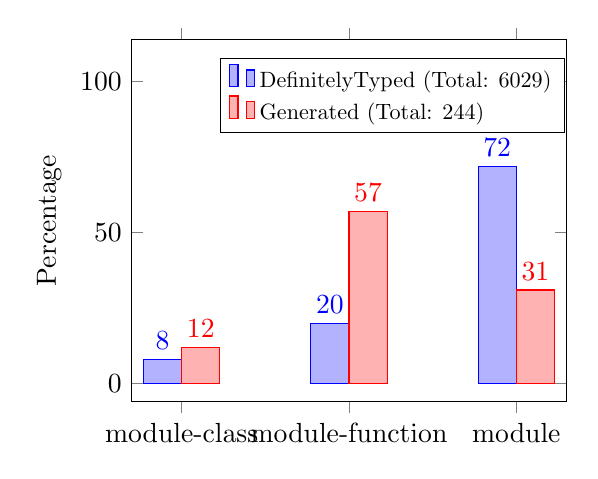
\begin{tikzpicture}
		\begin{axis}[
			ybar,
            width=0.7\textwidth,
            scale=0.8,
			ybar=0pt,
			ymax=100,
			enlargelimits=0.15,
			bar width=0.04\textwidth,
			legend columns=1,
			legend cell align={left},
			legend style={
                at={(0.6,0.95)},
                anchor=north,
                nodes={scale=0.8, transform shape}
            },
			symbolic x coords={module-class,module-function,module},
			xtick=data,
			ylabel=Percentage,
			nodes near coords, 
			nodes near coords align={vertical}
		]
		\addplot coordinates {
			(module-class, 8)
			(module-function, 20)
			(module, 72)
		};

		\addplot coordinates {
			(module-class, 12)
			(module-function, 57)
			(module, 31)
		};
		\legend{DefinitelyTyped (Total: 6029), Generated (Total: 244)}
		\end{axis}
	\end{tikzpicture}

	\caption[TypeScript templates distribution | Generated \& DefinitelyTyped]{\textbf{TypeScript templates distribution | Generated \& DefinitelyTyped} - Out of a total of 6029, 72\% of the modules uploaded to the DefinitelyTyped repository use the \lstinline{module} template and only 20\% use the \lstinline{module-function} one. However, 57\% of the 244 generated declaration files use the \lstinline{module-function} template.
	}

	\label{fig:experiments-typescript-templates-distribution-definitely-typed}
\end{figure}

\section{Related Work}
\paragraph*{Microsoft's dts-gen}
Microsoft developed \lstinline[language={}]{dts-gen}, a tool that creates starter declaration files for JavaScript libraries \cite{dts-gen}. Its documentation states that the result is however intended to be only used a starting point. The outcome needs to be refined afterwards by the developers.

The tool analyzes the shape of the objects at runtime after initialization without executing the library. This results in many variables being inferred as \lstinline[language={}]{any}. \coderef{code:related-work-dts-gen-example} shows an example for module \lstinline[language={}]{abs}.

The solution presented in this work, however, is intended to generate declaration files that are ready to be uploaded to DefinitelyTyped without further manual intervention. Any amount of manual work that a developer needs to do on a declaration file after updating JavaScript code increases the risk for having discrepancies between the declaration file and the implementation.

Formal aspects like applying the right template and using the correct syntax are perfectly covered by \lstinline[language={}]{dts-gen}.

\begin{lstlisting}[
    language=bash,
    caption={Microsoft's dts-gen example - A declaration file for module \lstinline!abs! is generated. Types are inferred as \lstinline!any!. The correct \lstinline!module-function! template is used.},
	label=code:related-work-dts-gen-example,
    float,
    abovecaptionskip=-\medskipamount
]
$ npm i -g dts-gen
$ npm i -g abs
$ dts-gen -m abs
Wrote 5 lines to abs.d.ts.

$ cat abs.d.ts
/** Declaration file generated by dts-gen */

export = abs;

declare function abs(input: any): any;
\end{lstlisting}

\paragraph*{TSInfer \& TSEvolve}
TSInfer and TSEvolve are presented as part of TSTools \cite{DBLP:conf/fase/KristensenM17}. Both tools are the continuation of TSCheck \cite{DBLP:conf/oopsla/FeldthausM14}, a tool for looking for mismatches between a declaration file and an implementation.

TSInfer proceeds in a similar way than TSCheck. It initializes the library in a browser and it records a snapshot of the resulting state and then it performs a light weight static analysis on all the functions and objects stored in the snapshot.

The abstraction and the constraints they introduced as part of the static analysis tools for inferring the types have room for improvement. A run-time based approach like the one presented in our work will provide more accurate information, thus generating more precise declaration files.

Since they analyze the objects and functions stored in the snapshot, they faced the problem of including in the declaration file internal methods and properties that developers wanted to hide. Run-time information would have informed that the developer has no intention of exposing such methods.

Moreover, TSEvolve performs a differential analysis on the changes made to a JavaScript library in order to determine intentional discrepancies between declaration files of two consecutive versions. We consider that a differential analysis may not be needed. If the developer's intention is accurately extracted and the execution code clearly represents that intention then the generated declaration file would already describe the newer version of a library without the need of a differential analysis.

\paragraph*{TSTest}
TSTest is a tool that checks for mismatches between a declaration file and a JavaScript implementation \cite{DBLP:journals/pacmpl/KristensenM17}. It applies feedback-directed random testing for generating type test scripts. These scripts will execute the library in order to check if it behaves the way it is described in the declaration file. TSTest also provides concrete executions for mismatches.

We evaluated the generated declaration files comparing them to the declaration files uploaded to DefinitelyTyped. The disadvantage of doing this is that since the uploaded files are written manually, they could already contain mismatches with the JavaScript implementation. However, it is a suitable choice for a development stage since it is used as a baseline.

In a final stage, declaration files need to be checked against the proper JavaScript implementation and TSTest has to be definitely taken into account.

\section{Conclusion}
We have presented \lstinline{dts-generate}, a tool for generating a TypeScript declaration file for a specific JavaScript library. The tool downloads code samples written by the developers from the library's repository. It uses these samples to execute the library and gather data flow and type information. The tool finally generates a TypeScript declaration file based on the information gathered at run-time.

We developed an architecture that supports the automatic generation of declaration files for specific JavaScript libraries without additional manual tasks. The architecture contemplates a future incorporation of a Symbolic Execution Engine that refines the initial code base enabling the exploration of new execution paths. However not implemented in this work, its incorporation would result in small incremental modifications to the presented architecture as it is considered to only expand the existing code base.

Building an end-to-end solution for the generation of TypeScript declaration files was prioritized over type inference accuracy. Consequently, types were taken over from the values at run-time. Since developers expose through code how a library should be used, obtaining the types from the code examples extracted from the repositories proved to be a pragmatic and effective approximation, enabling to work on specific aspects regarding the TypeScript declaration file generation itself.

We built a mechanism to automatically create declaration files for potentially every module uploaded to DefinitelyTyped. We managed to generate declaration files for 244 modules. We compared the results against the corresponding files uploaded to DefinitelyTyped by creating a TypeScript declaration files parser and a comparator.

We exposed the fundamental aspect of capturing the developer's intention when inferring types in JavaScript. Instead of applying constraints and restrictions for operations with certain types, we presented a proposal where common practices are favored. Uncommon usage is not forbidden but greatly disfavored. Accordingly, we collected evidence regarding the usage of JavaScript operators by analyzing 400 libraries.

Finally, the architecture is composed of different blocks that interact with each other. Each block is independent and has a well defined behavior as well as clear input and output values. As a result, each block can be independently and simultaneously improved.


\bibliography{lipics-v2019-sample-article}

\end{document}
